\begin{center}
\Huge
Bestemte integraler og arealer under grafer
\end{center}

\section*{Det bestemte integral}
\stepcounter{section}
Tidligere har vi defineret det ubestemte integral som en slags omvendt funktion til differentiation, og vi har set på forskellige egenskaber ved det ubestemte integral som linearitet. Vi skal nu betragte det bestemte integral, der er en evaluering af det ubestemte integral i intervalendepunkter. Vi starter med en definition.
\begin{defn}
Lad $f$ være en kontinuert funktion. Så definerer vi det bestemte integral fra $a$ til $b$ for $f$ som
\begin{align*}
\int_a^bf(x) dx = F(b)-F(a),
\end{align*}
hvor $F$ er en stamfunktion til $f$. 
\end{defn}
Det viser sig, at det bestemte integral meget overraskende tilsvarer arealet under grafen for funktionen $f$ på intervallet $[a,b]$ så længe $f$ er positiv og kontinuert på hele intervallet. Dette kan ses illustreret på 
Figur \ref{fig:areal}
\begin{figure}[H]
	\centering
	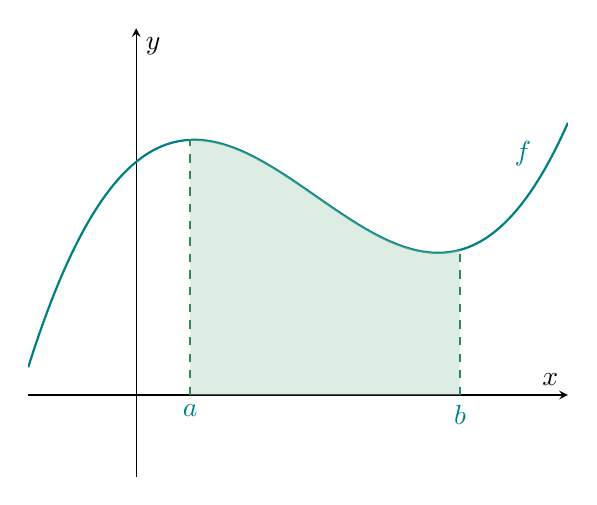
\begin{tikzpicture}
	\begin{axis}[
		axis lines = center, xmin = -2, xmax = 8,
		ymin = -1, ymax = 4.5,
		ticks = none, 
		xlabel = $x$,
		ylabel = $y$,
		]
			\addplot[color = teal, domain = -2:8, samples = 500, thick] {0.03*x^(3) - 0.3*x^(2) + 0.54*x + 2.86};
			\fill[color = SeaGreen!40, variable = \x, domain = 1:6,opacity = 0.4] (axis cs: 1,0) --
			 plot (axis cs: \x, 0.03*\x^3 - 0.3*\x^2 + 0.54*\x + 2.86) -- (axis cs: 6,0) -- cycle;
			 \draw[color = SeaGreen, dashed, thick] (axis cs: 1,0) -- (axis cs: 1,3.14);
			 \draw[color = SeaGreen, dashed, thick] (axis cs: 6,0) -- (axis cs: 6,1.78);
			 \node[color = teal, anchor = north] at (axis cs: 1,0) {$a$};
			 \node[color = teal, anchor = north] at (axis cs: 6,0) {$b$};
			 \node[color = teal, anchor = south east] at (axis cs: 7.5,2.69) {$f$};
	\end{axis}
	\end{tikzpicture}
	\caption{Areal under graf der tilsvarer det bestemte integral af funktionen på intervallet $[a,b]$.}
	\label{fig:areal}
\end{figure}
\newpage
\begin{setn}
For en kontinuert, ikke-negativ funktion $f$ er arealet afgrænset af $x$-aksen, to punkter $a$ og $b$ og grafen for $f$ givet ved
\begin{align*}
\int_a^bf(x) dx.
\end{align*} 
Dette areal tilsvarer det skraverede område på Figur \ref{fig:areal}.
\end{setn}
\begin{proof}
	For funktionen $f$ definerer vi funktionen $A_a(b)$, der giver arealet under grafen for $f$ på intervallet $[a,b]$. 
	Vi antager blot, at sådan en funktion eksisterer. Vi betragter så arealet fra $a$ til et punkt $x_0$ samt arealet
	fra $a$ til $x_0 + h$, hvor $h$ er et lille, positivt tal. Situationen kan ses på Figur \ref{fig:bevisareal}
	\begin{figure}[H]
		\centering
		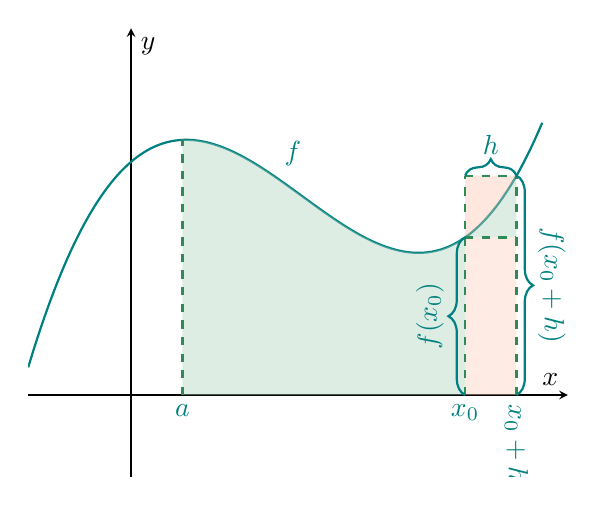
\begin{tikzpicture}
		\begin{axis}[
			axis lines = center, xmin = -2, xmax = 8.5,
			ymin = -1, ymax = 4.5,
			ticks = none, 
			xlabel = $x$,
			ylabel = $y$,
			]
				%Graf
				\addplot[color = teal, domain = -2:8, samples = 500, thick] {0.03*x^(3) - 0.3*x^(2) + 0.54*x + 2.86};
				%Areal indtil x0		
				\fill[color = SeaGreen!40, variable = \x, domain = 1:6.5,opacity = 0.4, samples = 500] (axis cs: 1,0) --
				 plot (axis cs: \x, 0.03*\x^3 - 0.3*\x^2 + 0.54*\x + 2.86) -- (axis cs: 6.5,0) -- cycle;
				 % Baggrund under f(x0)
			 	 \fill[
				 variable = \x,
				 domain = 6.5:7.5,
				 opacity = 0.4,
				 color = Melon!40
				 ] (axis cs: 6.5,0) --
			 	plot (axis cs: \x, 1.93375) -- (axis cs: 7.5,0) -- cycle;
			 	%Trekant over f(x0)
			 	\fill[color = SeaGreen!40, variable = \x, domain = 6.5:7.5,opacity = 0.4, samples = 500] 
			 	(axis cs: 6.5,1.93375) -- 
			 	plot (axis cs: \x, 0.03*\x^3 - 0.3*\x^2 + 0.54*\x + 2.86) --
			 	(axis cs: 7.5,1.93375) -- cycle;
			 	%Trekant under f(x0 + h)
			 	\fill[color = Melon!50, variable = \x, domain = 6.5:7.5,opacity = 0.4, samples = 500] 
			 	(axis cs: 7.5,2.69125) -- (axis cs: 6.5,2.69125) -- 
			 	plot (axis cs: \x, 0.03*\x^3 - 0.3*\x^2 + 0.54*\x + 2.86) -- cycle;
			 	%Dashes
			 	\draw[color = SeaGreen, dashed, thick] (axis cs: 1,0) -- (axis cs: 1,3.14);
			 	\draw[color = SeaGreen, dashed, thick] (axis cs: 6.5,0) -- (axis cs: 6.5,2.69125);
			 	\draw[color = SeaGreen, dashed, thick] (axis cs: 7.5,0) -- (axis cs: 7.5,2.69125);
			 	\draw[color = SeaGreen, dashed, thick] (axis cs: 6.5,1.93375) -- (axis cs: 7.5,1.93375);
			 	\draw[color = SeaGreen, dashed, thick] (axis cs: 6.5,2.69125) -- (axis cs: 7.5,2.69125);
			 	%Text
			 	\node[color = teal, anchor = north] at (axis cs: 1,0) {$a$};
			 	\node[color = teal, anchor = north] at (axis cs: 6.5,0) {$x_0$};
			 	\node[color = teal, anchor = south east] at (axis cs: 3.5,2.69) {$f$};
				 \node[color = teal, anchor = west, rotate = -90] at (axis cs: 7.5,0) {$x_0 + h$};
				 %Brace
				 \draw [decorate,decoration={brace,amplitude=6pt,mirror}, color = teal, thick]
				 (axis cs: 7.5,0) -- (axis cs: 7.5,2.69125) 
				 node[midway, anchor = south, rotate = -90, yshift = 4pt] {$f(x_0+h)$};
				 \draw [decorate,decoration={brace,amplitude=6pt}, color = teal, thick]	
				 (axis cs: 6.5,0) -- (axis cs: 6.5,1.93375) 
				 node[midway, anchor = south, rotate = 90, yshift = 4pt] {$f(x_0)$};
				 \draw [decorate,decoration={brace,amplitude=6pt}, color = teal, thick]
				 (axis cs: 6.5,2.69125) -- (axis cs: 7.5,2.69125) 
				 node[midway, anchor = south, yshift = 4pt] {$h$};
		\end{axis}
		\end{tikzpicture}
		\caption{Approksimation af areal under graf}
		\label{fig:bevisareal}
	\end{figure}
	Det må gælde, at det sande areal $A_a(x_0 + h)$ må være mindre end eller lig arealet op til $x_0$ lagt sammen med
	arealet af det store kvadrat på Figur \ref{fig:bevisareal}, altså at
	\begin{align*}
		A_a(x_0 + h) \leq A_a(x_0) + f(x_0 + h)h
	\end{align*}
	Tilsvarende må det sande areal $A_a(x_0 + h)$ være større end arealet op til $x_0$ lagt sammen emd det lille 
	kvadrat, altså
	\begin{align*}
		A_a(x_0) + f(x_0)h \leq A_a(x_0 + h).
	\end{align*}
	Samler vi disse uligheder, får vi
	\begin{align*}
		A_a(x_0) + f(x_0)h \leq A_a(x_0 + h) \leq A_a(x_0) + f(x_0 + h)h.
	\end{align*}
	Vi trækker nu $A_a(x_0)$ fra gennem hele udtrykket.
	\begin{align*}
		f(x_0)h \leq A_a(x_0 + h) - A_a(x_0) \leq f(x_0 + h)h.
	\end{align*}
	Afslutningsvist deler vi udtrykket med $h$.
	\begin{align*}
		f(x_0) \leq \frac{A_a(x_0 + h) - A_a(x_0)}{h} \leq f(x_0 + h).
	\end{align*}
	Her kan vi se, at det midterste udtryk tilsvarer differenskvotiententen for $A_a(x_0)$. Vi lader derfor $h \to 0$, 
	og vi får 
	\begin{align*}
		\lim_{h \to 0}f(x_0) \leq \lim_{h \to 0}\frac{A_a(x_0 + h)-A_a(x_0)}{h} \leq \lim_{h \to 0}f(x_0 + h).
	\end{align*}
	Da $f$ er antaget kontinuert, vil $\displaystyle\lim_{h\to 0}f(x_0 + h) = f(x_0)$, så vi har altså, at 
	\begin{align*}
		f(x_0) \leq \lim_{h \to 0}\frac{A_a(x_0 + h)-A_a(x_0)}{h} \leq f(x_0),
	\end{align*}
	men da det midterste udtryk både er mindre end eller lig og større end eller lig $f(x_0)$, så må det være lig 
	$f(x_0)$. Derfor har vi, at arealfunktionen $A_a$ er veldefineret og differentiabel og har differentialkvotienten
	\begin{align*}
		A_a'(x) = \lim_{h \to 0}\frac{A_a(x_0 + h)-A_a(x_0)}{h} = f(x).
	\end{align*}
	Dette må altså betyde, at $A_a$ er en stamfunktion til $f$, og vi har derfor for det bestemte integral, at
	\begin{align*}
		\int_{a}^b f(x) dx = A_a(b) - A_a(a) = A_a(b),
	\end{align*}
	og tilsvarer derfor arealet fra $a$ til $b$ under grafen for $f$. 
\end{proof}
Vi lægger ud med at betragte et eksempel, hvor vi kan verificere arealet under grafen med værktøjer, vi allerede er bekendte med.
\begin{exa}
Vi betragter funktionen $f$ givet ved
\begin{align*}
	f(x) = 2x + 3,
\end{align*}
og ønsker at bestemme arealet under grafen på intervallet $[2,4]$. Vi betragter grafen på Figur \ref{fig:trapez}.
\begin{figure}[H]
	\centering
	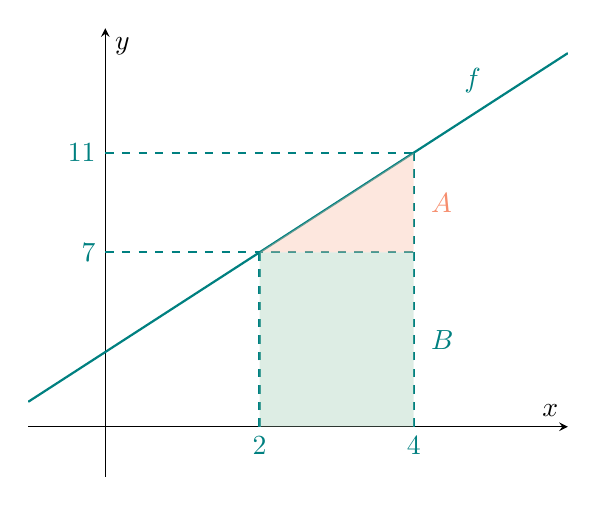
\begin{tikzpicture}
	\begin{axis}[
		axis lines = center, 
		xmin = -1, xmax = 6,
		ymin = -2, ymax = 16,
		ticks = none,
		xlabel = $x$, 
		ylabel = $y$, 
	]
		\addplot[color = teal, thick, domain = -1:6] {2*x + 3};	
		\draw[color = teal, thick, dashed] (axis cs: 2,0) -- (axis cs: 2,7);
		\draw[color = teal, thick, dashed] (axis cs: 4,0) -- (axis cs: 4,11);
		\draw[color = teal, thick, dashed] (axis cs: 0,7) -- (axis cs: 4,7);
		\draw[color = teal, thick, dashed] (axis cs: 0,11) -- (axis cs: 4,11);
		\fill
		[
			color = Melon!50,
			opacity = 0.4,
			variable = \x, 
			domain = 2:4,
		]	
			(axis cs: 4,7) -- (axis cs: 2,7) --
			plot(axis cs: \x, 2*\x + 3) --  cycle;
		\fill
		[
			color = SeaGreen!40,
			opacity = 0.4,
			variable = \x, 
			domain = 2:4,
		]	
			(axis cs: 4,0) -- (axis cs: 2,0) --
			plot(axis cs: \x, 7) --  cycle;
		\node[anchor = north, color = teal] at (axis cs: 2,0) {$2$};
		\node[anchor = north, color = teal] at (axis cs: 4,0) {$4$};
		\node[anchor = south east, color = teal] at (axis cs: 5, 13) {$f$};
		\node[anchor = east, color = teal] at (axis cs: 0, 11) {$11$};
		\node[anchor = east, color = teal] at (axis cs: 0, 7) {$7$};
		\node[anchor = west, color = teal] at (axis cs: 4.1, 3.5) {$B$};
		\node[anchor = west, color = Melon] at (axis cs: 4.1,9) {$A$};
	\end{axis}
	\end{tikzpicture}
	\caption{Areal under graf opdelt i trekant og rektangel.}
	\label{fig:trapez}
\end{figure}
Vi begynder ved at finde arealet som summen af arealerne $\color{Melon}{A}$ og $\color{teal}{B}$, der tilsvarer det trekantede område og firkantede
område på Figur \ref{fig:trapez} henholdsvis. Vi har derfor
\begin{align*}
	\color{Melon}{A} \color{black}= \frac{1}{2}\cdot 2 \cdot 4 = 4,
\end{align*}
og 
\begin{align*}
	\color{teal}{B} \color{black}= 2\cdot 7 = 14,
\end{align*}
så det totale areal er 
\begin{align*}
	\color{Melon} A \color{black} + \color{teal} B \color{black} = 18.
\end{align*}
Vi bestemmer nu arealet som et integral.
\begin{align*}
	\int_a^b f(x) dx &= \int_2^4 2x + 3 dx \\
	&= \left[x^2+3x \right]_2^4 \\
	&= \underbrace{4^2 + 3\cdot 4}_{F(4)} - \underbrace{(2^2+3\cdot 2)}_{F(2)} \\
	&= 16+12 - 4 - 6 = 18,
\end{align*}
og vi får altså også her arealet under grafen til at være 18.
\end{exa}

\subsection*{Opgave 1}
En funktion $f$ er givet ved
\begin{align*}
	f(x) = -x + 5.
\end{align*}
\begin{enumerate}[label=\roman*)]
	\item Bestem arealet under grafen for $f$ som set på Figur \ref{fig:opg1} ved brug af arealformler.
	\item Bestem arealet under grafen for $f$ som set på Figur \ref{fig:opg1} som et integral.
\end{enumerate}
\begin{figure}[H]
	\centering
	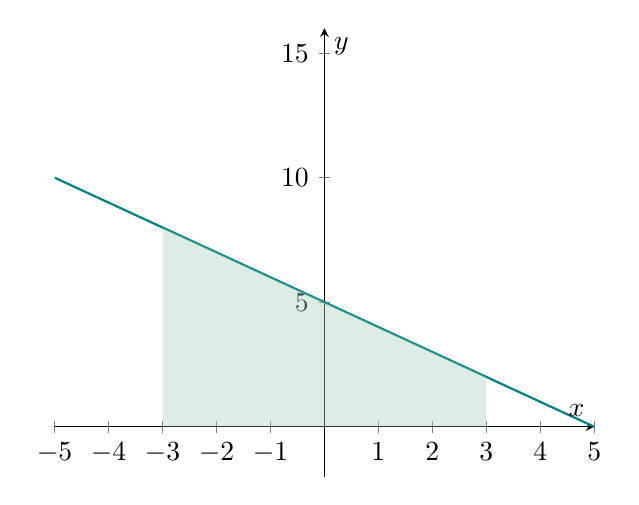
\begin{tikzpicture}
	\begin{axis}[
		axis lines = center, 
		xmin = -5, xmax = 5,
		ymin = -2, ymax = 16,
		xtick = {-5,-4,-3,...,3,4,5},
		xlabel = $x$, 
		ylabel = $y$, 
	]
		\addplot[color = teal, thick, domain = -5:5] {-x + 5};	
		\fill
		[
			color = SeaGreen!40,
			opacity = 0.4,
			variable = \x, 
			domain = -3:3,
		]	
			(axis cs: 3,0) -- (axis cs: -3,0) --
			plot(axis cs: \x, -\x + 5) --  cycle;
	\end{axis}
	\end{tikzpicture}
	\caption{Areal under $f$.}
	\label{fig:opg1}
\end{figure}

\newpage

\subsection*{Opgave 2}
En funktion $f$ er givet ved
\begin{align*}
	f(x) = 3x.
\end{align*}
\begin{enumerate}[label=\roman*)]
	\item Bestem arealet under grafen for $f$ som set på Figur \ref{fig:opg2} ved brug af arealformler.
	\item Bestem arealet under grafen for $f$ som set på Figur \ref{fig:opg2} som et integral.
\end{enumerate}
\begin{figure}[H]
	\centering
	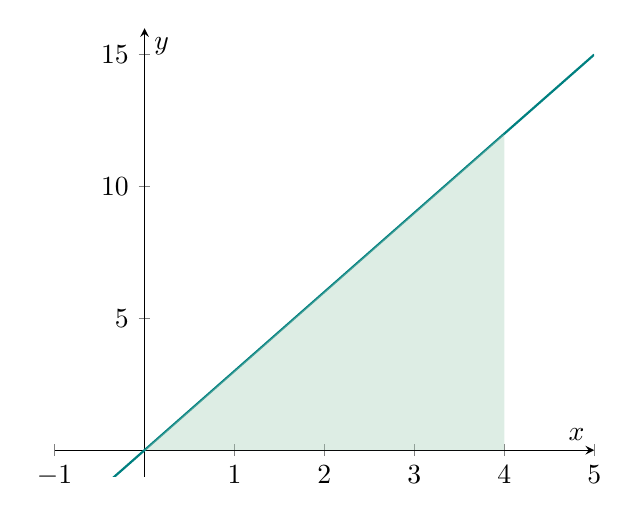
\begin{tikzpicture}
	\begin{axis}[
		axis lines = center, 
		xmin = -1, xmax = 5,
		ymin = -1, ymax = 16,
		xtick = {-5,-4,-3,...,3,4,5},
		xlabel = $x$, 
		ylabel = $y$, 
	]
		\addplot[color = teal, thick, domain = -1:5] {3*x};	
		\fill
		[
			color = SeaGreen!40,
			opacity = 0.4,
			variable = \x, 
			domain = 0:4,
		]	
			(axis cs: 4,0) -- (axis cs: 0,0) --
			plot(axis cs: \x, 3*\x) --  cycle;
	\end{axis}
	\end{tikzpicture}
	\caption{Areal under $f$.}
	\label{fig:opg2}
\end{figure}

\newpage

\subsection*{Opgave 3}
En funktion $f$ er givet ved
\begin{align*}
	f(x) = 
	\begin{cases}
		-2x + 9, \ &\textnormal{ hvis }x < 4, \\
		4x - 15, \ &\textnormal{ hvis }x \geq 4.
	\end{cases}	
\end{align*}
\begin{enumerate}[label=\roman*)]
	\item Bestem arealet under grafen for $f$ som set på Figur \ref{fig:opg3} ved brug af arealformler.
	\item Bestem arealet under grafen for $f$ som set på Figur \ref{fig:opg3} som et integral.
\end{enumerate}
\begin{figure}[H]
	\centering
	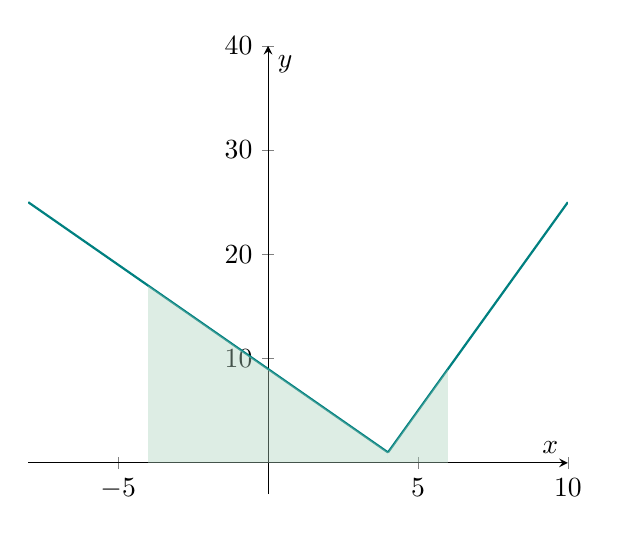
\begin{tikzpicture}
	\begin{axis}[
		axis lines = center, 
		xmin = -8, xmax = 10,
		ymin = -3, ymax = 40,
		xlabel = $x$, 
		ylabel = $y$, 
	]
		\addplot[color = teal, thick, domain = -8:4] {-2*x+9};
		\addplot[color = teal, thick, domain = 4:10] {4*x-15};	
		\fill
		[
			color = SeaGreen!40,
			opacity = 0.4,
			variable = \x, 
			domain = -4:4,
		]	
			(axis cs: 4,0) -- (axis cs: -4,0) --
			plot(axis cs: \x, -2*\x+9) --  cycle;
			\fill
		[
			color = SeaGreen!40,
			opacity = 0.4,
			variable = \x, 
			domain = 4:6,
		]	
			(axis cs: 6,0) -- (axis cs: 4,0) --
			plot(axis cs: \x, 4*\x-15) --  cycle;
	\end{axis}
	\end{tikzpicture}
	\caption{Areal under $f$.}
	\label{fig:opg3}
\end{figure}

\newpage

\subsection*{Opgave 4}
Grafen for funktionen $f$ kan ses på Figur \ref{fig:opg4}. Funktionen $f$ er givet ved
\begin{align*}
	f(x) = \frac{1}{2}x^3 - 2x^2 + x + 4.
\end{align*}
\begin{enumerate}[label=\roman*)]
	\item Bestem arealet af det farvede område på Figur \ref{fig:opg4}.
\end{enumerate}
\begin{figure}[H]
	\centering
	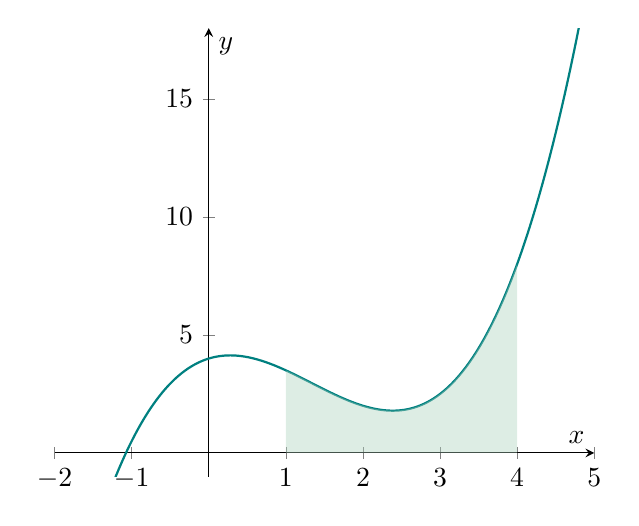
\begin{tikzpicture}
	\begin{axis}[
		axis lines = center, 
		xmin = -2, xmax = 5,
		ymin = -1, ymax = 18,
		xtick = {-5,-4,-3,...,3,4,5},
		xlabel = $x$, 
		ylabel = $y$, 
	]
		\addplot[color = teal, thick, domain = -3:5, samples = 500] {0.5*x^3 - 2*x^2 + x + 4};	
		\fill
		[
			color = SeaGreen!40,
			opacity = 0.4,
			variable = \x, 
			domain = 1:4,
			samples = 500,
		]	
			(axis cs: 4,0) -- (axis cs: 1,0) --
			plot(axis cs: \x, 0.5*\x^3-2*\x^2+\x+4) --  cycle;
	\end{axis}
	\end{tikzpicture}
	\caption{Areal under $f$.}
	\label{fig:opg4}
\end{figure}

\newpage
\subsection*{Opgave 5}
To grafer $f$ og $g$ kan ses på Figur \ref{fig:opg5}. Funktionerne er givet ved henholdsvis
\begin{align*}
	f(x) = \frac{1}{10}x^3 - \frac{1}{5}x^2 - \frac{1}{2}x + 2,
\end{align*}
og 
\begin{align*}
	g(x) = x + 2.
\end{align*}
\begin{enumerate}[label=\roman*)]
	\item Bestem arealet af det farvede område på Figur \ref{fig:opg5}.
\end{enumerate}
\begin{figure}[H]
	\centering
	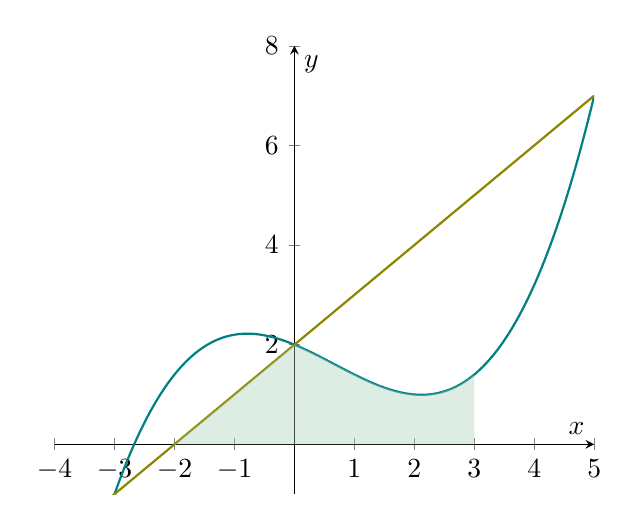
\begin{tikzpicture}
	\begin{axis}[
		axis lines = center, 
		xmin = -4, xmax = 5,
		ymin = -1, ymax = 8,
		xtick = {-5,-4,-3,...,3,4,5},
		xlabel = $x$, 
		ylabel = $y$, 
	]
		\addplot[color = teal, thick, domain = -4:5, samples = 500] {0.1*x^3 - 0.2*x^2 - 0.5*x + 2};
		\addplot[color = olive, thick, domain = -4:5, samples = 500] {x + 2};	
		\fill
		[
			color = SeaGreen!40,
			opacity = 0.4,
			variable = \x, 
			domain = -2:0,
			samples = 500,
		]	
			(axis cs: 0,0) -- (axis cs: -2,0) --
			plot(axis cs: \x, \x + 2) --  cycle;
			\fill
		[
			color = SeaGreen!40,
			opacity = 0.4,
			variable = \x, 
			domain = 0:3,
			samples = 500,
		]	
			(axis cs: 3,0) -- (axis cs: 0,0) --
			plot(axis cs: \x, 0.1*\x^3 - 0.2*\x^2 - 0.5*\x + 2) --  cycle;
	\end{axis}
	\end{tikzpicture}
	\caption{Areal under $f$ og $g$.}
	\label{fig:opg5}
\end{figure}


\subsection*{Opgave 6}
Udregn følgende bestemte integraler
\begin{align*}
	&1) \ \int_0^2 3x^2-1 dx   &&2) \ \int_{-3}^3 x^3  dx    \\
	&3) \ \int_{-3}^2 2x^2-5x + 3 dx  &&4) \ \int_1^{e^2} \frac{5}{x} dx    \\
\end{align*}
